\section{Analyse von Funktion F220: Ausleihe}
\label{f:220}
Ein oder mehrere Dokumente werden von einem Benutzer ausgeliehen. Dabei wählt 
der Benutzer das gewünschte Dokument aus und das System muss in der Datenbank 
nachprüfen, ob dieses derzeit ausleihbar ist. Wenn dies der Fall sein sollte, 
wird dem Benutzer dieses Buch zugewiesen. Dies erfolgt durch zwei 
Built-In-Funktionen von \gls{glos:django}, mit dessen Hilfe die Datenbank 
erweitert bzw.\ ein Datensatz geupdatet werden kann. Es gehört zum 
\textbf{View}-Komponent im Zusammenhang zur \textbf{DB}.

Das Sequenzdiagramm ist strukturell das selbe wie Abb.\ \ref{fig:221}. Es muss 
nur keine Eingabe von \gls{glos:ext}n getätigt werden. Daher entfallen die 
Schritte 1.1 und 1.2. 

\section{Analyse von Funktion F221: Ausleihe an Externe}
\label{f:221}
Die Ausleihe an \gls{glos:ext} ist ähnlich gestaltet wie in \ref{f:220} 
\nameref{f:220} und gehört ebenfalls dem \textbf{View}-Komponent mit 
\textbf{DB}-Einflüssen. Es existiert lediglich der Zusatz, dass der Benutzer 
einen \gls{glos:ext}n als eigentlichen Ausleiher angibt. Dafür wird beim 
Entleihen die Möglichkeit gegeben, Daten über den \gls{glos:ext}n anzugeben, 
dessen Daten dann gespeichert und beim Entleihen vermerkt werden. Auch hierbei 
wird eine Built-In-Funktion zum Erweitern der Datenbank genutzt.

Das Sequenzdiagramm der Abb. \ref{fig:221} ist nur der Hauptteil. Vorher müsste 
erst eine Suchanfrage getätigt werden (wie in Abb.\ \ref{fig:F-A}) bzw.\ eine 
Überprüfung, ob das gewünschte Dokument derzeit vorhanden ist. Außerdem sei 
erwähnt, dass nach jedem Schritt, falls ein Fehler aufgetreten sein sollte, eine 
Fehlermeldung ausgegeben wird.

\begin{figure}
\begin{center}
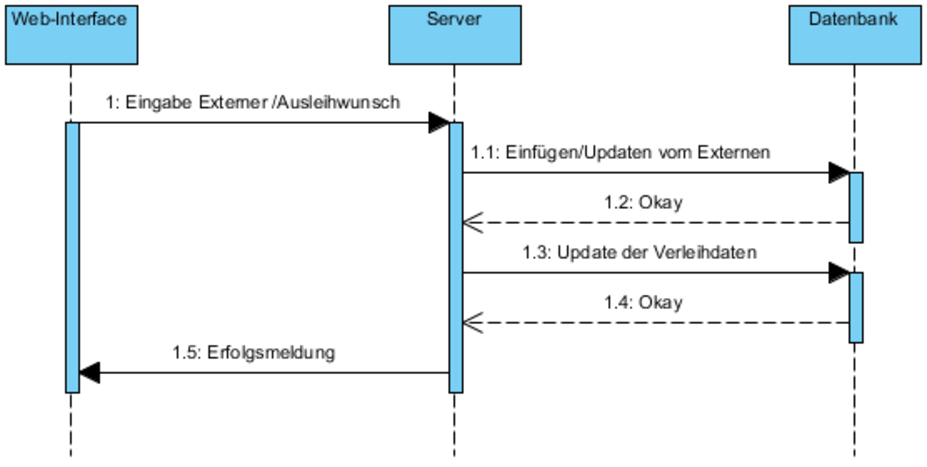
\includegraphics[width=0.8\linewidth]{bilder/Seq-Ausleihe.pdf}
\caption{Sequenzdiagramm für Ausleihe an Externe}
\label{fig:221}
\end{center}
\end{figure}

\section{Analyse von Funktion F222: Ausleihe übertragen}
\label{f:222}
Ein Dokument wechselt den Ausleihenden. Dabei muss ein Benutzer $A$ ein von ihm 
ausgeliehenes Dokument auswählen und einem anderen Benutzer $B$ übertragen. 
Alternativ kann Benutzer $B$ auch eintragen, dass er sich ein Dokument von 
Benutzer $A$ geholt hat, das Dokument also jetzt bei ihm zu finden ist. Das 
System vermerkt dieses Austausch dann in der Datenbank mittels einer 
Built-In-Funktion von \gls{glos:django}. Auch diese gehört zur 
\textbf{View}-Komponente mit Zugriff auf die \textbf{DB}.

Auch dieses Sequenzdiagramm ist strukturgleich mit Abb.\ \ref{fig:221}. Bei 
dieser Funktion muss vorher allerdings geprüft werden, ob das Dokument wirklich 
ausgeliehen ist (auch nur eine Suchanfrage wie in Abb.\ \ref{fig:F-A}). Außerdem 
entfällt wieder die Eingabe von \gls{glos:ext}n (Schritte 1.1 und 1.2).

\section{Analyse von Funktion F223: Ausleihe zurückgeben}
\label{f:223}
Ein Benutzer braucht ein Dokument nicht mehr und gibt es in den Bestand der 
Bibliothek zurück. Auch hierfür muss der Benutzer als Entleiher des Dokumentes 
eingetragen sein. Wenn dies der Fall sein sollte, kann er \emph{zurückgeben} 
wählen und das Dokument wird auch im Datensatz mittels Built-In-Funktionen von 
\gls{glos:django} mit dem Status 0 versehen. Die Funktion ist dem \textbf{View} 
zugeordnet, benötigt aber auch die \textbf{DB}.

Wieder ist die Struktur wie bei Abb. \ref{fig:221} vorzufinden. Hierbei muss 
vorher geprüft werden, ob der Benutzer auch wirklich das Dokument ausgeliehen 
hat (Suchanfrage nach Abb.\ \ref{fig:F-A}. Die Schritte 1.1 und 1.2 zur 
\gls{glos:ext}nausgabe wird wieder weggelassen.

\section{Analyse von Funktion F224: Ausleihe vermisst melden}
\label{f:224}
Das Dokument befindet sich nicht mehr an dem laut Datenbank befindlichen Ort. 
Dann kann ein Benutzer ein Dokument auf der Dokumentenansicht als 
\emph{vermisst} melden und dieses wird in der Datenbank mittels Statusänderung 
vermerkt. Dazu wird eine E-Mail an alle Benutzer verschickt oder alternativ eine
Meldung auf der Homepage angezeigt. Hierfür stellt \gls{glos:django} wieder 
Built-In-Funktionen bereit. Das Ganze gehört dann zu \textbf{View} und 
\textbf{DB}.

Das dazugehörige Sequenzdiagramm ist Abb.\ \ref{fig:224}.
\begin{figure}
\begin{center}
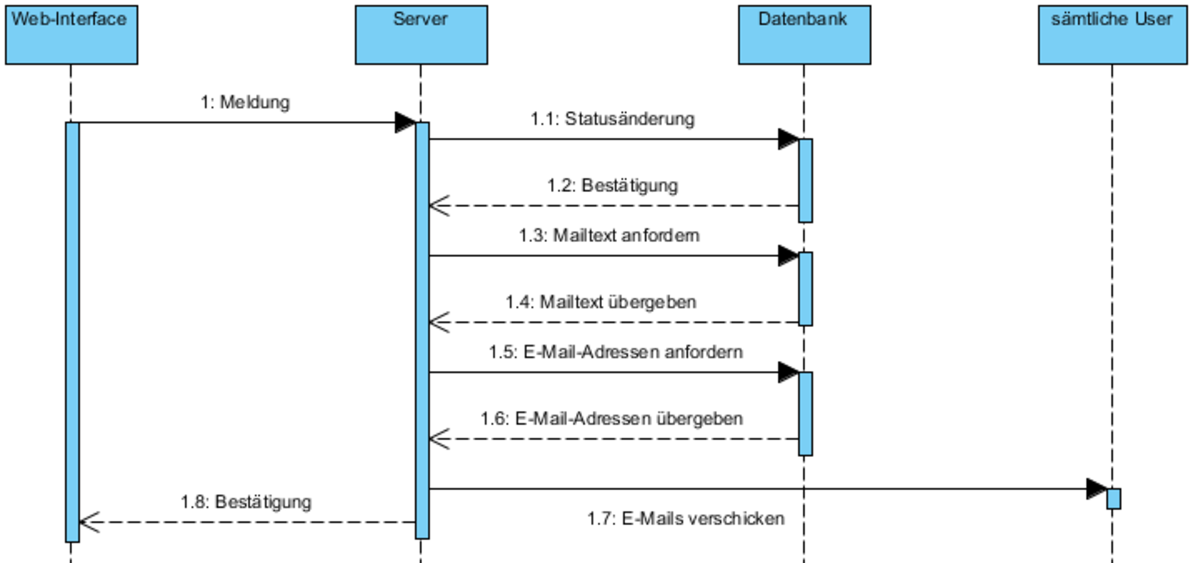
\includegraphics[width=0.8\linewidth]{bilder/Seq-Vermisst.pdf}
\caption{Sequenzdiagramm für eine Vermisstmeldung}
\label{fig:224}
\end{center}
\end{figure}

\section{Analyse von Funktion F225: Ausleihe verloren melden}
\label{f:225}
Das Dokument ist auch nach einer Vermisstenmeldung nicht wieder aufgetaucht. 
Dann ist ein Bibliothekar berechtigt, es als \emph{verloren gegangen} 
einzustufen. Das Dokument bekommt den entsprechenden Status und wird demnächst 
bei weiteren Suchanfragen ausgeschlossen. Dies erfolgt wieder innerhalb der 
\textbf{View}- und \textbf{DB}-Komponenten durch eine Built-In-Funktion von 
\gls{glos:django}.

Das gewünschte Sequenzdiagramm ist strukturell gleich dem von Abb.\ 
\ref{fig:224}. Dabei muss nur vorher geprüft werden, ob der Nutzer die 
entsprechenden Rechte besitzt (Abb.\ \ref[{fig:F-A}), und Schritt 1.3 bis 1.7 
entfällt, da keine E-Mails verschickt werden.
